\documentclass{standalone}
\usepackage{pgfplots}
\pgfplotsset{compat=1.7}

\begin{document}
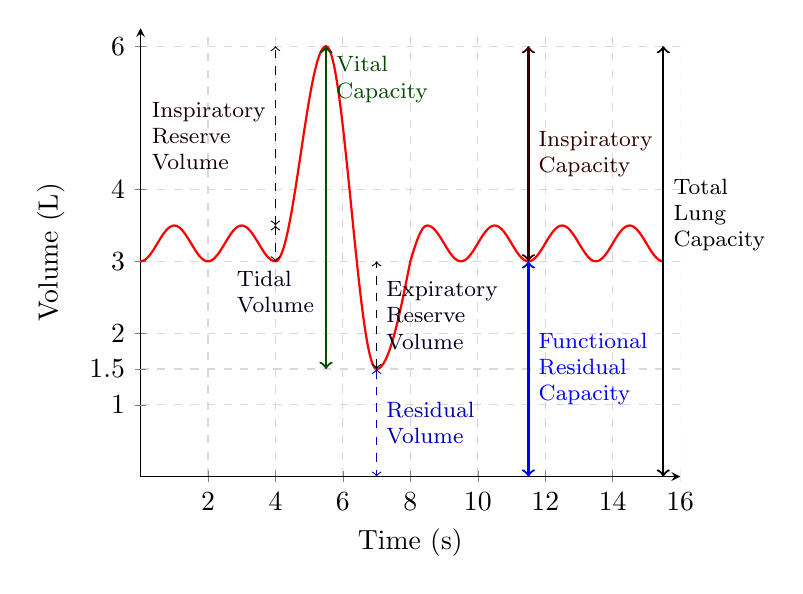
\begin{tikzpicture}
    \begin{axis}[
        axis x line=middle,
        axis y line=middle,
        grid = major,
        grid style={dashed, gray!30},
	extra y ticks={1, 1.5, 3},
extra y tick labels={1, 1.5,3},
        xmin=0,
        xmax= 16,
        ymin= 0,
        ymax= 6.25,
	 ylabel near ticks,
	xlabel near ticks,
        xlabel=Time (s),
        ylabel=Volume (L),
clip=false]

  \draw[thick, red]
	(axis cs: 0, 3) cos (axis cs: 0.5,3.25) sin (axis cs: 1, 3.5) cos (axis cs: 1.5,3.25) sin (axis cs: 2,3) cos (axis cs: 2.5,3.25) sin (axis cs: 3,3.5) cos (axis cs: 3.5,3.25) sin (axis cs: 4,3)
	cos (axis cs: 4.75, 4.5) sin (axis cs: 5.5, 6) cos (axis cs: 6.25, 3.75) sin (axis cs: 7, 1.5) cos (axis cs: 8, 3)
 sin (axis cs: 8.5, 3.5) cos (axis cs: 9, 3.25) sin (axis cs: 9.5, 3) cos (axis cs: 10, 3.25) sin (axis cs: 10.5, 3.5) cos (axis cs: 11, 3.25) sin (axis cs: 11.5, 3)
cos (axis cs: 12, 3.25) sin (axis cs: 12.5, 3.5) cos (axis cs: 13, 3.25) sin (axis cs: 13.5, 3.0) cos (axis cs: 14, 3.25) sin (axis cs: 14.5, 3.5) cos (axis cs: 15, 3.25) sin (axis cs:  15.5, 3);


\draw[dashed, blue!70!black,<->] (axis cs: 7,1.5) -- node[right,blue!70!black,font=\footnotesize, align=left]{Residual \\ Volume}(axis cs: 7,0);
\draw[dashed, blue!10!black,<->] (axis cs: 7,1.5) -- node[right,blue!10!black,font=\footnotesize, align=left]{Expiratory \\ Reserve \\ Volume}(axis cs: 7,3);
\draw[dashed, red!10!black,<->] (axis cs: 4,3.5) -- node[left,red!10!black,font=\footnotesize, align=left]{Inspiratory \\ Reserve \\ Volume}(axis cs: 4,6);
\draw[dashed, black,<->] (axis cs: 4,3.5) -- (axis cs: 4,3) node[below,blue!10!black,font=\footnotesize, align=left]{Tidal \\ Volume};


\draw[blue,thick,<->] (axis cs: 11.5,0) -- node[right,blue,font=\footnotesize, align=left]{Functional  \\ Residual \\ Capacity}(axis cs: 11.5,3);
\draw[red!20!black,thick,<->] (axis cs: 11.5,3) -- node[right,red!20!black,font=\footnotesize, align=left]{Inspiratory \\ Capacity}(axis cs: 11.5,6);
\draw[green!30!black, thick, <->] (axis cs: 5.5,1.5) -- (axis cs: 5.5,6) node[below right,green!30!black,font=\footnotesize, align=left]{Vital \\ Capacity};
\draw[black,thick,<->] (axis cs: 15.5,0) -- node[above right,black,font=\footnotesize, align=left]{Total \\ Lung \\ Capacity}(axis cs: 15.5,6);

\end{axis}


\end{tikzpicture} 
\end{document}